\apendice{Especificación de diseño}

\section{Introducción}
En esta sección se describir el diseño de la aplicación GreenInHouse 2.0, desarrollada para gestionar mejor el cuidado de las plantas mediante el uso de sensores.
La aplicación ha sido diseñado mediante la integración con herramientas previamente creadas por el autor del primer proyecto GreenInHouse, Oscar Valverde Escobar, ya que ha sido necesaria la interacción entre la API REST y la aplicación para poder trabajar con los datos guardados en la base de datos.

El diseño se ha creado teniendo en cuenta los requisitos funcionales previamente creados en la anterior sección del proyecto.

\section{Diseño de datos}
El diseño de datos de la aplicación se basa en los datos recogidos de la base de datos previamente creada por el autor del primer proyecto GreenInHouse.
De esta manera la aplicación puede trabajar con los datos recogidos de los sensores como con los datos almacenados sobre las plantas.

La aplicación no accede directamente a la base de datos, si no que deberá comunicarse con ella a través de la API REST la cual permitirá realizar las llamadas a los diferentes endpoints ya sea para obtener información de la base de datos como para modificarla. La información de la base de datos también puede ser modificada o eliminada a través de la aplicación mediante diferentes pantallas que sirven para la creación, modificación o eliminación de plantas creadas. 

El diseño del flujo de datos que tiene el proyecto es el siguiente:\ref{D1}:
\begin{figure}[H]
    \centering
    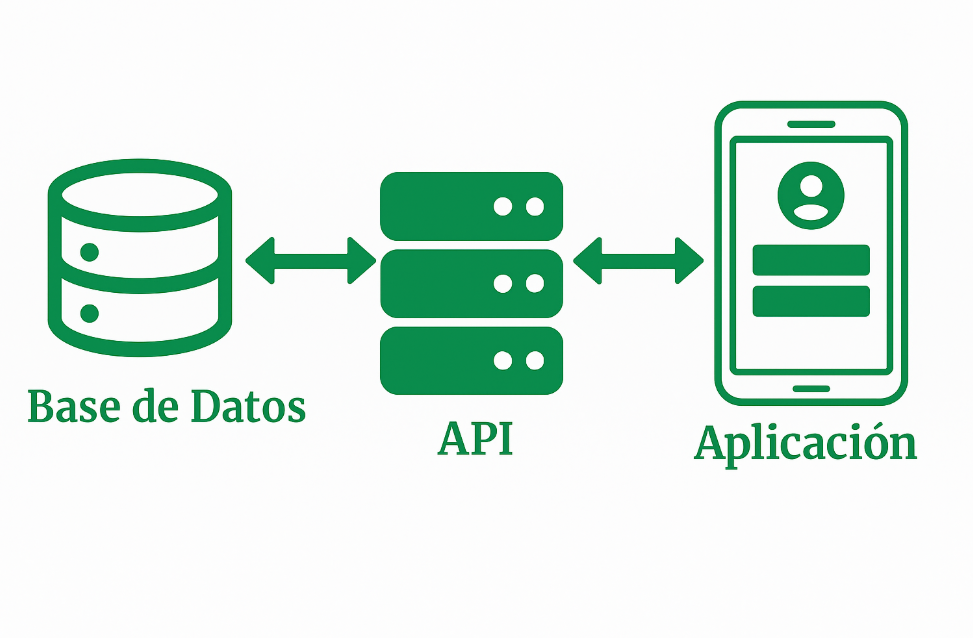
\includegraphics[width=0.8\linewidth]{Intercambio_Datos.png}
    \caption{Diseño de Datos}
    \label{D1}
\end{figure}



\section{Diseño arquitectónico}
En cuanto al diseño arquitectónico, nos referimos como la manera en que se organiza y estructura un proyecto, en este caso la aplicación GreenInHouse 2.0.

Este diseño muestra cómo el usuario interactúa con la interfaz de la aplicación ya sea para llevar a cabo alguna acción en la que interviene también la interacción con la base de datos a través de la API como alguna acción que no requiera de dicha comunicación con la API como por ejemplo, cambiar el idioma de la aplicación.

Para este proyecto se ha seguido una arquitectura basada en el patrón Modelo-Vista-Controlador(MVC) extendido con una capa de servicios usada para la gestión de los datos a través de una API:
\begin{enumerate}
    \item \textbf{Modelo:}
   Se refiere a las clases de datos que se usan en la aplicación de GreenInHouse 2.0 como pueden ser:
    \begin{enumerate}
        \item {Planta}
        \item {Sensor}
        \item {Consejo}
    \end{enumerate}
    \item \textbf{Vista:}
    Se refiere a las pantallas con los que el usuario va a interactuar en la aplicación como pueden ser:
    \begin{enumerate}
        \item {Pantalla de Gráficos}
        \item {Pantalla de Hitos}
        \item {Pantalla de Inicio}
        \item {Pantalla de Ajustes}
    \end{enumerate}
    \item \textbf{Controlador:}
    Se refiere a la lógica que hay detrás de cada acción realizada por el usuario como puede ser:
    \begin{enumerate}
        \item {Cambio de Idioma}
        \item {Creación de Planta}
        \item {Cambio de Tierra}
    \end{enumerate}
    \item \textbf{Servicio:}
    Se refiere a todas esas llamadas HTTP(GET, POST, PUT, DELETE) que el usuario puede realizar las cuales actúan de intermediario entre la lógica del programa y la API.
\end{enumerate} 

Para que este diseño arquitectónico sea completamente funcional se va a necesitar que haya conexión a internet. Dependiendo de si hay conexión a internet o no se van a dar los siguientes casos:
\begin{enumerate}
    \item \textbf{Con Internet:}
    La mayoría de las funcionalidades de la aplicación dependen de la comunicación con la base de datos a través de la API. Para ello se va a necesitar que tanto la maceta como el teléfono móvil estén conectados a la misma red. Estas funcionalidades incluyen:
    \begin{enumerate}
        \item {Consulta de Sensores}
        \item {Consulta de Gráficos}
        \item {Consulta de Consejos}
        \item {Crear Plantas}
        \item {Editar Plantas}
        \item {Eliminar Plantas}
    \end{enumerate}
    \item \textbf{Sin Internet:}
    Sin esta conexión a internet la aplicación va a ser parcialmente funcional y entre estas cosas están:
    \begin{enumerate}
        \item {La interfaz carga sin problema}
        \item {Los datos guardados en el archivo ``SharedPreferences'' si que se usan.}
        \item {Funciones que no requieran de la API como el cambio de idioma}
    \end{enumerate}
\end{enumerate}


\section{Diseño procedimental}
A diferencia del diseño de arquitectura que se basaba en conocer la organización de la aplicación, el diseño procedimental se centra en ver cómo se comporta la aplicación durante su ejecución y uso. Va a mostrar la interacción entre el usuario y la aplicación y los resultados a las decisiones tomadas en tiempo de ejecución.

A continuación se verán ejemplos de diseños procedimentales de las diferentes acciones posibles dentro de la aplicación:

\subsection{Creación de una Planta:}
    \begin{enumerate}
        \item {El usuario abre la aplicación.}
        \item {Accede a la pantalla de creación de plantas.}
        \item {Rellena los campos necesarios y pulsa el botón crear planta.}
        \item {El sistema valida los campos.}
        \item {Si son válidos se envía una petición POST a la API y en caso contrario te da error y vuelves al paso 3.}
        \item {La planta se crea y queda registrada en la base de datos.}
    \end{enumerate}

\subsection{Consulta de Hitos Diarios:}
    \begin{enumerate}
        \item {El usuario abre la aplicación.}
        \item {Accede a la pantalla de hitos.}
        \item {Se hace una petición GET a la API para que devuelva tanto los datos recogidos por los sensores como los de los consejos.}
        \item {El sistema compara los datos recogidos por los sensores con los de los consejos y determina el estado del hito}
    \end{enumerate}
    
\subsection{Consulta de Gráficos:}
    \begin{enumerate}
        \item {El usuario abre la aplicación.}
        \item {Accede a la pantalla de gráficos.}
        \item {Se hace una petición GET a la API para que devuelva tanto los datos recogidos por los sensores como los de los consejos.}
        \item {El sistema compara los datos recogidos por los sensores con los de los consejos y determina el estado del gráfico}
    \end{enumerate}
    
\subsection{Consulta de Sensores:}
    \begin{enumerate}
        \item {El usuario abre la aplicación.}
        \item {Accede a la pantalla de comprobar sensores.}
        \item {Se hace una petición GET a la API para que devuelva el estado de los sensores}
    \end{enumerate}
\subsection{Modificación de una Planta:}
    \begin{enumerate}
        \item {El usuario abre la aplicación.}
        \item {Accede a la pantalla de modificar planta.}
        \item {Selecciona el tipo de planta y el nombre de la planta a modificar.}
        \item {El sistema valida los campos.}
        \item {Si son válidos se envía una petición PUT a la API y en caso contrario te da error y vuelves al paso 3.}
        \item {La planta se modifica y queda registrada en la base de datos.}
    \end{enumerate}
\subsection{Eliminación de una Planta:}
    \begin{enumerate}
        \item {El usuario abre la aplicación.}
        \item {Accede a la pantalla de eliminar planta.}
        \item {Selecciona la planta a eliminar y pulsa el botón eliminar planta.}
        \item {El sistema valida los campos.}
        \item {Si son válidos se envía una petición DELETE a la API y en caso contrario te da error y vuelves al paso 3.}
        \item {La planta se elimina de plantas activas en la base de datos y se registra como planta marchita.}
    \end{enumerate}